\chapter{\huge Metodo Implicito}

\textit{Per sistemi di equazioni alle derivate parziali (PDE) esistono altri metodi oltre a quelli RK. In questa sezione si illustra e implementa il cosidetto metodo implicito per risolvere equazioni agli operatori lineari.}

\begin{figure}[H]
\centering
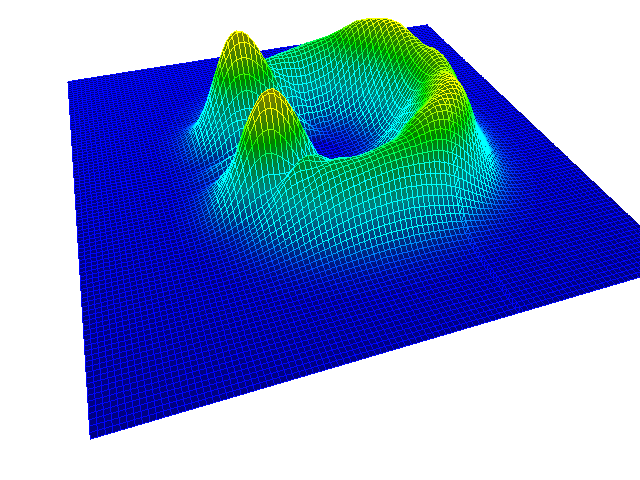
\includegraphics[width=\textwidth]{schrodinger}
\caption{Scattering di un pacchetto gaussiano con una buca di potenziale. L'onda, arrivando da destra, scattera contro la buca di potenziale posta al centro del reticolo senza riuscire ad attraversarla.}
\label{fig:schrodinger}
\end{figure}

\section{Equazione di Schr\"{o}dinger}

L'equazione che si intende risolvere è l'equazione di Schr\"odinger dipendente dal tempo
$$i\hbar\frac{\partial}{\partial t} \psi(x,\,t) = -\frac{\hbar^2}{2m}\nabla^2\psi(x,\,t) + V(x)\psi(x,\,t)$$
A tal fine si discretizza lo spazio in modo tale che $x=na$, con $n=0,...,N-1$, ed $a$ passo del reticolo spaziale. $\psi(x,\,t)$ diventa quindi un vettore di valori complessi $\psi_n(t)$. Si pongono inoltre condizioni di periodicità al contorno di modo che $\psi_N \equiv \psi_0$.

Con questa dicretizzazione si sostituisce
$$\nabla^2\psi(x) \rightarrow \frac{\psi_{n+1}+\psi_{n-1}-2\psi_n}{a^2} $$
pertanto l'equazione diventa
$$i\hbar\frac{\partial}{\partial t} \psi_n = -\frac{\hbar^2}{2m}\frac{\psi_{n+1}+\psi_{n-1}-2\psi_n}{a^2} + V_n\psi_n = \sum\limits_{n}A_{n,m}\psi_m$$
La soluzione dell'equazione è la funzione esponenziale
$$\psi(t)=\exp\left(-\frac{i}{\hbar}At\right)\psi(0)$$
dove $U(t) = \exp(-\frac{i}{\hbar}At)$ rappresenta l'evolutore temporale del sistema. Sviluppando ora $U(t)$ intorno all'unita per $t\rightarrow 0$ e trascurando gli ordini superiori in $t$ si ottiene la formula approssimata
$$\psi(t_0+t)\simeq\psi(t_0)-\frac{i}{\hbar}At\psi(t_0)$$
Questa prima approssimazione tuttavia porta all'insorgere di numerosi problemi dovuti al fatto che l'iterazione descritta dal precedente passaggio non rispetta la condizione di unitarietà dell'operatore evolutore temporale. Bisogna quindi ricorrere ad una strategia più astuta.

Il \textbf{metodo implicito}~\cite{cinque} consiste nell'approssimare l'operatore esatto $U(t)$ attraverso la formula
$$\psi(t+dt)=(1+\frac{i}{2\hbar}Adt)^{-1}(1-\frac{i}{2\hbar}Adt)\psi(t)$$
Utilizzando il fatto che $A$ è Hermitiano, è facile dimostrare che l'operatore della precedente formula è unitario proprio come $U(t)$.
Per implementare questo algoritmo è necessario risolvere ad ogni step il sistema lineare
$$(1+\frac{i}{2\hbar}Adt)\psi(t+dt)=(1-\frac{i}{2\hbar}Adt)\psi(t)$$

Infine si moltiplicano entrambi i membri dell'equazione per l'aggiunto dell'operatore a primo membro, in modo tale da ottenere
$$(1+\frac{1}{4\hbar^2}A^2dt^2)\psi(t+dt)=(1-\frac{i}{2\hbar}Adt)^2\psi(t)$$
dove ora $(1+\frac{1}{4\hbar^2}A^2dt^2)$ è Hermitiano e si può quindi risolvere rispetto a $\psi(t+dt)$ utilizzando il \textit{Conjugate Residual Method}~\cite{tre}.\\

L'idea che sta alla base di questo metodo è che se in un intervallo di tempo $dt$ la funzione $\psi(t)$ evolve in $\psi(t+dt)$, allora facendo evolvere $\psi(t)$ in avanti nel tempo per $\frac{dt}{2}$ e $\psi(t+dt)$ indietro nel tempo sempre di $\frac{dt}{2}$ le due funzioni dovranno necessariamente coincidere.
\\

Al fine di migliorare la precisione dell'approssimazione è anche possibile utilizzare sviluppi a ordini superiori in $t$ al costo, tuttavia, di incrementare considerevomente la complessità dell'algoritmo. L'unitarietà dell'operatore è evidentemente preservata ad ogni ordine proprio grazie a come è stata costruita l'approssimazione.
\\

La formula per l'evolutore al secondo ordine è data da
$$\psi(t+dt)=\left(1+\frac{i}{2\hbar}Adt-\frac{1}{8\hbar^2}A^2dt^2\right)^{-1}\left(1-\frac{i}{2\hbar}Adt-\frac{1}{8\hbar^2}A^2dt^2\right)\psi(t)$$
che svolgendo il procedimento descritto per lo sviluppo al primo ordine diventa
$$\left(1+\frac{1}{64\hbar^4}A^4dt^4\right)\psi(t+dt)=\left(1-\frac{i}{2\hbar}Adt-\frac{3}{8\hbar^2}A^2dt^2+\frac{i}{16\hbar^3}A^3dt^3+\frac{1}{64\hbar^4}A^4dt^4\right)\psi(t)$$

